\chapter{Nasazení}

\section{Softwarové požadavky}

Aplikace běží na virtualizovaném serveru s OS Ubuntu verze 15.10. Na veřejné adrese virtulního serveru
je dostupná RESTová webová služba Catcher, s níž může zvnějšku komunikovat libovolná aplikace,
která disponuje HTTP protokolem a dostupností běžného portu 80. Jako prostředník mezi klientskou aplikací
a uWSGI 2.0.12, jehož úkolem je udržovat Catchera, zde běží webový server Nginx 1.9.3.
Data se ukládají na databázový server MySQL verze 5.6.28.

\begin{figure}[ht!]
\centering
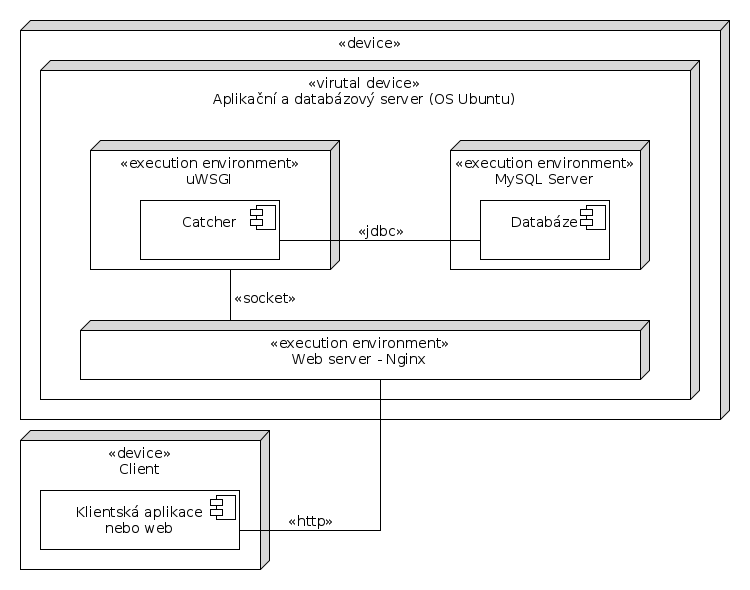
\includegraphics[width=130mm]{./images/diagram-nasazeni.png}
\caption{Diagram nasazení\label{overflow}}
\end{figure}

\section{Konfigurace}

Po získání přístupu na VPS jsem kromě výše zmíněných programů doinstaloval všechny potřebné balíčky nutné pro běh aplikace.
Mezi nimi šlo například o pip. Pro lepší správu systému jsem stáhnul mc.

Konfigurace nginx serveru ukazka configu:
Na webovem serveru mam zaroven jinou domenu nachystanou na dokumentace!

Spusteni uwsgi ulohy v pozadi: ukazat radek co dela.

Bylo potreba vytvorit uzivatele db s novym heslem a pravy, a to ulozit do konfiguracniho souboru, ktery jsem stahnul pres wget z meho soukromeho cloudoveho uloziste. Duvod, proc nebyl na gitu je ten, ze zadna hesla nesmi byt verejne dostupna. 

jak jsem ho vytvoril:

CREATE USER 'catcher-XXXXXXserver'@'localhost' IDENTIFIED BY 'tajne_heslo';
GRANT SELECT, INSERT, UPDATE, DELETE ON catcher. * TO 'catcher-XXXXXXserver'@'localhost';

%Co bylo potřeba udělat na serveru za činnosti. Co vsechno jsem nainstaloval apod. Muzu vychazet z meho souboru /server

Co všechno jsem musel nainstalovat na VPS.

Na VPS se nachazí...

Pro lepsi pouziti jsem mohl pouzit VIRTUALENV


\section{Údržba}

Zálohování databáze,

Nebyla na to kapacita, ale použil bych Cron (pod carou co to je), aby automaticky pravidelne informoval o nebezici aplikaci a zaroven aby dumpoval databazi pravidelne.

V budoucnu bych mohl jeste pouzit nastroje jako Codevoc (to je mozna spis testovani) nebo Travis CI.

% TODO: IDEA: Lze se zminit o testovani a prubezne integraci. Napriklad napsat, ze mame zajem v budoucnu pouzivat Codevoc nebo Travis CI.